\documentclass[eng,printmode,oneside,openany]{mgr2} %openany openright
%pakiety dodające dużo dodatkowych poleceń matematycznych
\usepackage{amsmath}
\usepackage{amsfonts}

\usepackage[polish]{babel}%alternatywnie do pakietu polski, wybrać jeden z nich
\usepackage{polski} %przydatne podczas składania dokumentów w j. polskim

%\usepackage[utf8x]{inputenc} %kodowanie znaków, zależne od systemu
%\usepackage{polski} %przydatne podczas składania dokumentów w j. polskim
%\usepackage[cp1250]{inputenc} %kodowanie znaków, zależne od systemu
%\usepackage[T1]{fontenc} %poprawne składanie polskich czcionek
%pakiety do grafiki
\usepackage[utf8]{inputenc} %kodowanie znaków, zależne od systemu
\usepackage{lmodern}
\usepackage[T1]{fontenc} %poprawne składanie polskich czcionek
\usepackage{ucs}
%\usepackage[MeX]{polski}
\usepackage{graphicx}
\usepackage{subfigure}
\usepackage{psfrag}

%pakiety wspomagające i poprawiające składanie tabel
\usepackage{supertabular}
\usepackage{array}
\usepackage{tabularx}
\usepackage{hhline}
\usepackage{listings}

\usepackage{float}
\usepackage{indentfirst}
\usepackage{color}
\usepackage{enumerate}

\usepackage{setspace}
\usepackage{tabularx}
\usepackage{color,calc}
\usepackage{listings}


\usepackage{wrapfig}
\usepackage{lscape}
\usepackage{rotating}
\usepackage{epstopdf}
%\usepackage{soul} % pakiet z komendami do podkreślania tekstu

\usepackage{ebgaramond} % pakiet z czcionkami garamond, potrzebny tylko do strony tytułowej, musi wystąpić przed pakietem tgtermes
%\usepackage[left=2.5cm,right=2.5cm,top=2.5cm,bottom=2.5cm]{geometry}
\topmargin -10mm

%% Aby uzyskać polskie literki w pdfie (a nie zlepki) korzystamy z pakietu czcionek tgterms. 
%% W pakiecie tym są zdefiniowane klony czcionek Times o kształtach: normalny, pogrubiony, italic, italic pogrubiony.
%% W pakiecie tym brakuje czcionki o kształcie: slanted (podobny do italic). 
%% Jeśli w dokumencie gdzieś zostanie zastosowana czcionka slanted (np. po użyciu komendy \textsl{}), to
%% latex dokona podstawienia na czcionkę standardową i zgłosi to w ostrzeżeniu (warningu).
%% Ponadto tgtermes to czcionka do tekstu. Wszelkie matematyczne wzory będą sformatowane domyślną czcionką do wzorów.
%% Jeśli wzory mają być sformatowane z wykorzystaniem innych czcionek, trzeba to jawnie zadeklarować.

%% Po zainstalowaniu pakietu tgtermes może będzie trzeba zauktualizować informacje 
%% o dostępnych fontach oraz mapy. Można to zrobić z konsoli (jako administrator)
%% initexmf --admin --update-fndb
%% initexmf --admin --mkmaps

\usepackage{tgtermes} 

%pakiet wypisujący na marginesie etykiety równań i rysunków zdefiniowanych przez \label{}, chcąc wygenerować finalną wersję dokumentu wystarczy usunąć poniższą linię
%\usepackage{showlabels} 
	
%definicje własnych poleceń
\newcommand{\R}{I\!\!R} %symbol liczb rzeczywistych, działa tylko w trybie matematycznym
\newtheorem{theorem}{Twierdzenie}[section] %nowe otoczenie do składania twierdzeń
\newcommand{\lssetdef}{\lstset{
		backgroundcolor=\color[rgb]{0.9,0.9,0.9},
		basicstyle={\small\ttfamily},
		breaklines=true,
		frame=l,
		tabsize=2,
		basicstyle=\small,
		xleftmargin={0.75cm},
		numbers=left,
		stepnumber=1,
		firstnumber=1,
		numberfirstline=true,
		showspaces=false,                % show spaces everywhere adding particular underscores; it overrides 'showstringspaces'
		showstringspaces=false,          % underline spaces within strings only
		showtabs=false,                  % show tabs within strings adding particular underscores
		language=SQL,
		inputencoding=utf8x, 
		extendedchars=true,
		literate={ą}{{\k{a}}}1
		{Ą}{{\k{A}}}1
		{ę}{{\k{e}}}1
		{Ę}{{\k{E}}}1
		{ó}{{\'o}}1
		{Ó}{{\'O}}1
		{ś}{{\'s}}1
		{Ś}{{\'S}}1
		{ł}{{\l{}}}1
		{Ł}{{\L{}}}1
		{ż}{{\.z}}1
		{Ż}{{\.Z}}1
		{ź}{{\'z}}1
		{Ź}{{\'Z}}1
		{ć}{{\'c}}1
		{Ć}{{\'C}}1
		{ń}{{\'n}}1
		{Ń}{{\'N}}1
}}

%dane do złożenia strony tytułowej
\project{Projektowanie systemów z dostępem w języku naturalnym}
\title{Opracowanie algorytmu określającego możliwe zamienniki dla błędnych słów w tekstach
	w języku polskim}
\engtitle{}
\author{Radosław Taborski - 209347\\Piotr Konieczny - 209174}
\supervisor{dr inż. Dariusz Banasiak}
%\guardian{dr hab. inż. Imię Nazwisko Prof. PWr, I-6} %nie używać jeśli opiekun jest tą samą osobą co prowadzący pracę

%\date{2017} %standardowo u dołu strony tytułowej umieszczany jest bieżący rok, to polecenie pozwala wstawić dowolny rok

%poniżej jest lista kierunków i specjalności na wydziale elektroniki, należy wybrać właściwe lub dopisać jeśli nie ma odpowiednich
\field{Informatyka (INF)}
\specialisation{Inżynieria systemów informatycznych (INS)}

%tutaj zaczyna się właściwa treść dokumentu
\begin{document}
	%\bibliographystyle{unsrt} %tylko gdy używamy BibTeXa, ustawia polski styl bibliografii
	
	\maketitle %polecenie generujące stronę tytułową
	
	%TODO: ten fragment do wersji archiwalnej
	%\newpage 
	%\thispagestyle{empty}
	%\ 
	%\newpage	

	\setcounter{page}{2}
	\tableofcontents %spis treści
	
	
	\linespread{1.2}
	%opcjonalnie może się tu pojawić spis rysunków i tabel
	\listoffigures
	\addcontentsline{toc}{chapter}{Spis rysunków} %utworzenie w spisie treści pozycji Spis rysunków
	
	\chapter{Wstęp}

\section{Cele projektu}

Głównym celem projektu jest stworzenie aplikacji, która będzie umożliwiała wpisanie przez użytkownika dowolnego tekstu w języku polskim oraz pozwoli na jego sprawdzenie pod względem użycia poprawnych słów. Następnie użytkownik będzie miał możliwość wstawienia za każde z wychwyconych błędnych wyrazów, innego, jednego z tych, które będą sugerowane przez aplikację, bądź też zignorowania sugestii. Aplikacja wyposażona będzie w algorytm sprawdzający czy wyraz istnieje w słowniku języka polskiego, gdy takiego nie znajdzie, wyszukiwane będą słowa o podobnej budowie, lecz nie koniecznie pasujące znaczeniowo do kontekstu zdania.

\section{Założenia projektowe}

W projekcie użyty został język programowania C\#, z wykorzystaniem technologii WPF, umożliwiającej tworzenie graficznego interfejsu użytkownika w oparciu o składnię XAML.

W projekcie wykorzystany został również słownik języka polskiego dostępny na stronie słownika języka polskiego [\ref{bib:slownik}]. Słownik ten zawiera podstawowe formy słów wraz ze wszystkimi możliwymi odmianami. Słownik ten przewiduje jedynie słowa o maksymalnej długości wynoszącej 15 znaków i nie zawiera żadnych nazw własnych tzn. imion, nazw krajów, miast itp.

\section{Zakres projektu}
Zakres projektu dotyczy zaprojektowania i implementacji aplikacji umożliwiającej pisanie własnych tekstów, które na bieżąco są sprawdzane pod względem poprawności ortograficznej.

Umożliwione użytkownikowi zostało również wklejanie gotowych tekstów, w celu ich sprawdzenia.

Projekt został wyposażony w trzy algorytmy umożliwiające uzyskanie podpowiedzi dla użytkownika oraz opracowane zostały sposoby optymalizacji tak, aby aplikacja działała w czasie rzeczywistym mimo słownika, który zawiera prawie 3 miliony pozycji.

\section{Opis rozdziałów}
\begin{enumerate}
	\item Rozdział I – opisuje założenia wstępne oraz zawiera informacje, na temat tego co projekt powinien zawierać. Rozdział ten ponadto stanowi wstęp, w którym zawarte są opisy wszystkich rozdziałów niniejszego dokumentu.
	\item Rozdział II – zawiera opis użytych w projekcie algorytmów wraz z diagramami.
	\item Rozdział III – opisuje fazę  projektową oraz szczegóły implementacyjne projektu oraz opis użytych metod przyśpieszających działanie programu.
	\item Rozdział IV – podsumowanie projektu wraz z analizą osiągniętych celów.
\end{enumerate}





	\chapter{Opis użytych algorytmów}
Projekt został wyposażony w trzy algorytmy wyszukujące słów podobnych pod względem budowy dla bazowego ciągu znaków, który nie występuje w użytym słowniku. 

\section{Odległość Levenshteina} \label{chap:Lev}
Pierwszym z użytych algorytmów jest algorytm na obliczanie długości Levenshteina (edycyjnej) [\ref{bib:Lev}]. Odległość ta jest miarą odmienności napisów. W algorytmie tym wyróżnia się takie pojęcie jak działanie proste na napisie. Do działań takich zaliczamy:
\begin{itemize}
	\item wstawienie nowego znaku do napisu;
	\item usunięcie znaku z napisu;
	\item zamianę znaku w napisie na inny znak;
\end{itemize}

Idea algorytmu polega na stworzeniu dwuwymiarowej tablicy, o wymiarach n+1 na m+1, gdzie n i m to długości porównywanych słów. Pierwszy wiersz i kolumna uzupełniane są wartościami odpowiedni od 0 do n i m. W następnym etapie po kolei bierze się wartości wiersza i porównuje literę dotyczącą tego wiersza z literą dotyczącą kolumny. Dokonuje się porównania na zasadzie każdy z każdym. Jeżeli litery są identyczne to ustawia się koszt na 0, jeśli nie to na 1. Następnie daną komórkę wypełnia się wartością, którą jest minimum z poniższych trzech pozycji:
\begin{itemize}
	\item wartości komórki leżącej bezpośrednio nad aktualnie badaną komórką zwiększoną o 1;
	\item wartości komórki leżącej bezpośrednio w lewo od naszej aktualnej komórki + 1;
	\item wartości komórki leżącej bezpośrednio w lewą-górną stronę od aktualnej komórki + koszt;
\end{itemize}
Po wykonaniu wszystkich porównań, odległością edycyjną będzie wartość w komórce~[n+1,~m+1]. Szczegółowy diagram działania został przedstawiony na rysunku~\ref{fig:Lev-Count}. \\

Algorytm ten posłużył w projekcie do przeszukiwania wybranych fragmentów słownika i wybierania tych słów, których odległość Levenshteina nie przekracza odległości podanej przez użytkownika w jednym z parametrów dostępnych w interfejsie aplikacji. Diagram przedstawiający wykorzystanie odległości Levenshteina został zademonstrowany na rysunku~\ref{fig:Lev}.

\begin{figure} [H]
	\centering
	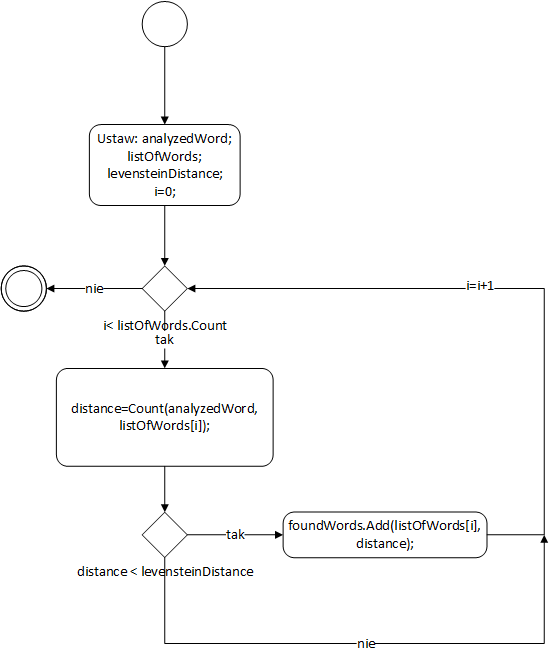
\includegraphics[width=0.8\linewidth]{rozdzial02/Levenstein1.png}
	\caption{Diagram działania algorytmu z wykorzystaniem odległości Levenshteina}
	\label{fig:Lev}
\end{figure}

\begin{figure} [H]
	\centering
	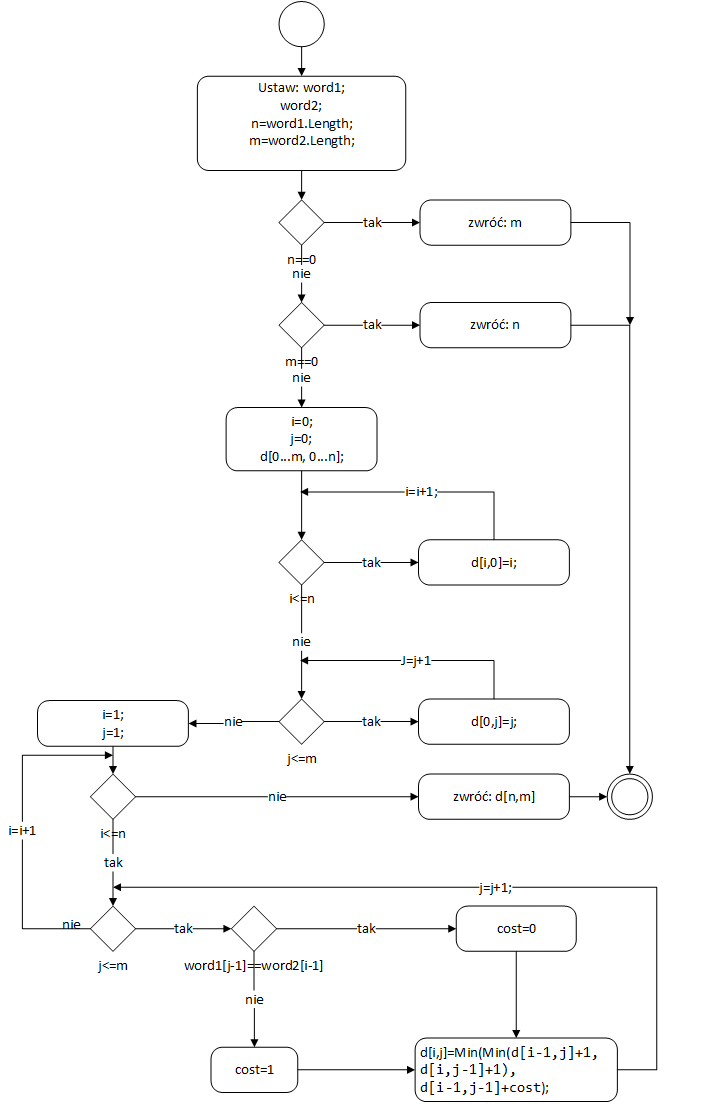
\includegraphics[width=1\linewidth]{rozdzial02/Levenstein-Count.png}
	\caption{Diagram obliczania odległości Levenshteina}
	\label{fig:Lev-Count}
\end{figure}


\section{Zamiana znaków}
\label{chap:Letter}
Ten algorytm do swojego działania potrzebuje listy najczęściej popełnianych błędów ortograficznych ([\ref{bib:ort}]). Wybrane ciągi znaków i ich odpowiedniki ustawione zostały w liście \_letterPairs, której elementy są typu KeyValuePair, składającego się z elementów jak Key i Value (oba są typu string), co przedstawione zostało na listingu~\ref{lst:letter}. Są to według autorów projektu ciągi znaków, w których najczęściej popełniane zostają błędy ortograficzne. 

\lssetdef
\lstinputlisting[captionpos=b,caption={Lista par ciągów znakowych odpowiadająca najczęstszym błędom w języku polskim},label={lst:letter},basicstyle={\footnotesize\ttfamily}]{rozdzial02/letterPairs.txt}

Badany ciąg znaków, zostaje sprawdzony pod względem obecności ciągów znaków, z powyższej listy, z parametru Key. Następnie badany ciąg znaków zostaje przekształcany poprzez zamienianie wszystkich ,,podejrzanych o błąd'' fragmentów na ich zamienniki, czyli na ciągi znaków z parametru Value. Na przykład ciąg znaków ,,grzegrzółka'', pod wpływem zamian wynikających z pierwszego elementu listy \_letterPairs może przyjąć następujące trzy formy: ,,gżegrzółka'', ,,grzegżółka'' oraz ,,gżegżółka''. Wszystkie te trzy formy zostają wychwycone przez algorytm i zwrócone do przeanalizowania w dalszym etapie programu. Przy okazji tego ciągu znaków, badane są również wszystkie ciągi znaków z uwzględnieniem zamiany ,,a'' na ,,ą'' oraz ,,e'' na ,,ę'', czyli m.in. powstają też takie kombinacje jak ,,gżęgrzółką'', ,,grzegrzółką''.  Gdyby badany ciąg znaków tworzył ,,grzegrzulka'' to dodatkowo znalezione byłyby wszystkie kombinacje zamieniające ,,u'' na ,,ó'' oraz ,,l'' na ,,ł''. Algorytm ten powstał w celu łatwiejszego znajdywania tych kombinacji, których ilość podstawowych zamian na napisie, opisanych w poprzednim podrozdziale~\ref{chap:Lev}, może sugerować, że zostało wykonanych wiele operacji, a tak na prawdę został popełniony np. jeden bądź dwa błędy ortograficzne, dobrym przykładem jest tutaj zamiana ,,cz'' na ,,trz''. Również biorąc pod uwagę, że z powodów optymalizacyjnych, przy mierzeniu odległości Levenshteina, nie jest badany cały słownik, a jedynie najbardziej prawdopodobne jego fragmenty (więcej w podrozdziale~\ref{chap:optym}), ten algorytm doskonale wychwytuje pozostałe nieprawidłowości w badanym ciągu znaków. Schemat działania tego algorytmu został przedstawiony na diagramie z rysunku~\ref{fig:LetterChanger}. Algorytm ten znajduje więc dość dużo różnych ,,dziwnych'' kombinacji, jednak w dalszym etapie wszystkie te kombinacje podlegają sprawdzeniu, czy występują w słowniku i na tej podstawie określane jest czy zostaną podpowiedziane użytkownikowi czy też nie.

\begin{figure} [H]
	\centering
	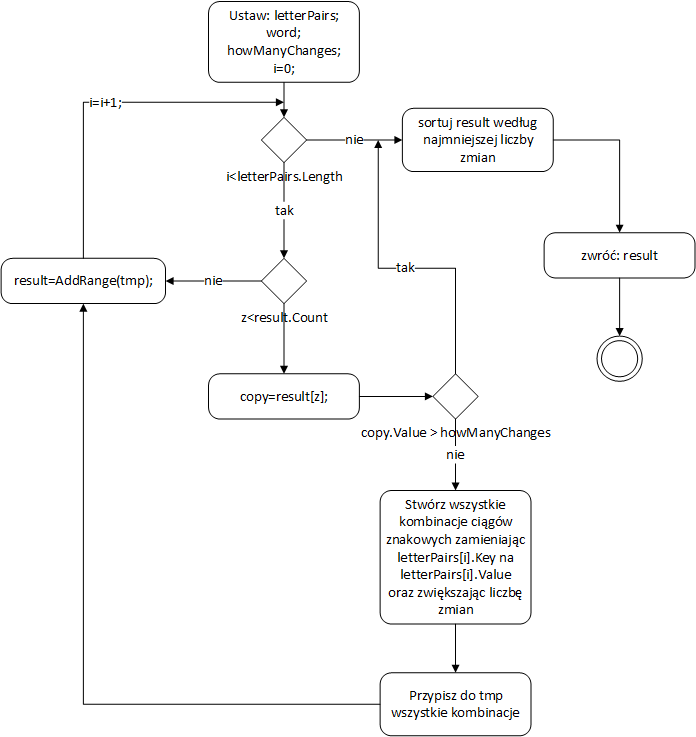
\includegraphics[width=1\linewidth]{rozdzial02/LetterChanger.png}
	\caption{Diagram zamieniania ciągów znaków odpowiadających najczęstszym błędom ortograficznym}
	\label{fig:LetterChanger}
\end{figure}

\section{Podział na wyrazy}
Algorytm ten powstał w celu wychwytywania, błędów, które na co dzień nie mają miejsca w piśmie ręcznym, jednak są powszechnym problemem w podczas opracowywania tekstów na komputerze. Mianowicie problem ten dotyczy braku wciśnięcia, bądź też reakcji komputera na wciśnięcie klawisza spacji. Algorytm ten bierze pod uwagę, że w jednym ciągu znakowym może wystąpić tylko jedno takie zdarzenie. Na przykład między innymi z ciągu znaków ,,idziekot'' zostanie przekształcony do postaci ,,idzie kot'', ale również do postaci ,,idzi ekot''. Algorytm ten nie tworzy zbyt wielu kombinacji, jednak rozwiązuje dość często popełniany błąd w pisowni komputerowej. Dodatkowo w dalszym etapie działania programu, kombinacje uzyskane z tego algorytmu podlegają też zamianom w oparciu o algorytm LetterChanger opisanym w podrozdziale~\ref{chap:Letter}, dzięki czemu również znajdywane są sugestie dla słów, w których popełniony został błąd ortograficzny oraz zabrakło spacji. Jednak kombinacja tych dwóch algorytmów niesie ze sobą ryzyko, iż znalezione zostaną dwa słowa, których kombinacja nie ma sensu w języku polskim, bądź też są błędnie odmienione względem siebie. Diagram UML, dla tego algorytmu został przedstawiony na grafice~\ref{fig:SpaceAdder}. 

\begin{figure} [H]
	\centering
	
\includegraphics[width=0.6\linewidth]{rozdzial02/SpaceSearcher.png}
	\caption{Diagram działania funkcji dodającej przerwy między wyrazami}
	\label{fig:SpaceAdder}
\end{figure}




	\chapter{Projekt i implementacja aplikacji}

\section{Funkcje aplikacji - diagram przypadków użycia}

\begin{figure} [H]
	\centering
	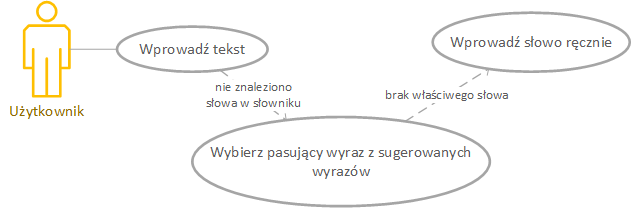
\includegraphics[width=1\linewidth]{rozdzial03/diagram.png}
	\caption{Diagram przypadków użycia}
	\label{fig:diagUzycia}
\end{figure}

Głównym zadaniem aplikacji jest wyszukiwanie błędnych wyrazów w języku polskim oraz ich korekcja. Aby tego dokonać aplikacja porównuje wyrazy znajdujące się w tekście z wyrazami znajdującymi się w słowniku. Jeśli danego słowa nie znaleziono zostaje ono uznane za błędne. Aby dokonać korekcji błędnych wyrazów stosowane są algorytmy opisane w poprzednich rozdziałach. Dla optymalizacji działania aplikacji wyszukiwanie sugestii odbywa się w osobnych wątkach co znacząco przyspiesza działanie aplikacji. 


\section{Interfejs aplikacji}

\begin{figure} [H]
	\centering
	\includegraphics[width=1\linewidth]{rozdzial03/screen1_1.png}
	\caption{Interfejs aplikacji}
	\label{fig:interfejs}
\end{figure}

\begin{enumerate}
	\item Ilość podpowiedzi - pozwala na ustawienie maksymalnej ilości podpowiedzi jakie mają się pojawić po kliknięciu prawym przyciskiem myszy na błędnie napisane słowo.
	\item Odległość Levenshteina - pozwala na ustawienie odległości jaka ma być brana pod uwagę w przypadku algorytmu Levenshteina. Im większa liczba tym więcej podpowiedzi ale jednocześnie zmniejsza to szybkość działania aplikacji ze względu na dodatkowe obliczenia które muszą zostać wykonane. 
	\item Ilość zmian - pozwala na ustawienie parametru ilości zmian dla algorytmu podmieniającego znaki diakrytyczne. Im większa liczba tym więcej podpowiedzi oraz dłuższy czas wykonywania algorytmu.
	\item Edytor tekstu - pozwala na edycję tekstu. Wyszukiwanie błędów działa w czasie rzeczywistym (funkcja sprawdzająca poprawność uruchamia się z każdym kliknięciem spacji). Jeśli dane słowo zostało uznane za błędne zostaje zaznaczone kolorem czerwonym. Aby je poprawić należy kliknąć na nie prawym przyciskiem myszki. Zostanie wyświetlone menu kontekstowe zawierające możliwe zamienniki. Aby podmienić słowo wystarczy kliknąć na zamiennik. Możliwe jest również poprawienie tekstu ręcznie wpisując w miejscu błędnego słowa poprawne. 
	
\end{enumerate}

\section{Wpływ parametrów na wyniki wyszukiwania}

\begin{figure} [H]
	\centering
	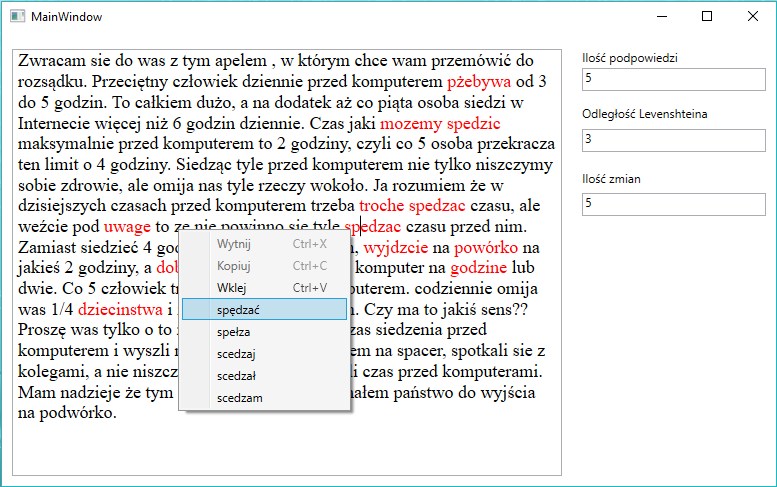
\includegraphics[width=1\linewidth]{rozdzial03/screen2.png}
	\caption{Przykładowy wynik wyszukiwania sugestii}
	\label{fig:interfejs1}
\end{figure}

\begin{figure} [H]
	\centering
	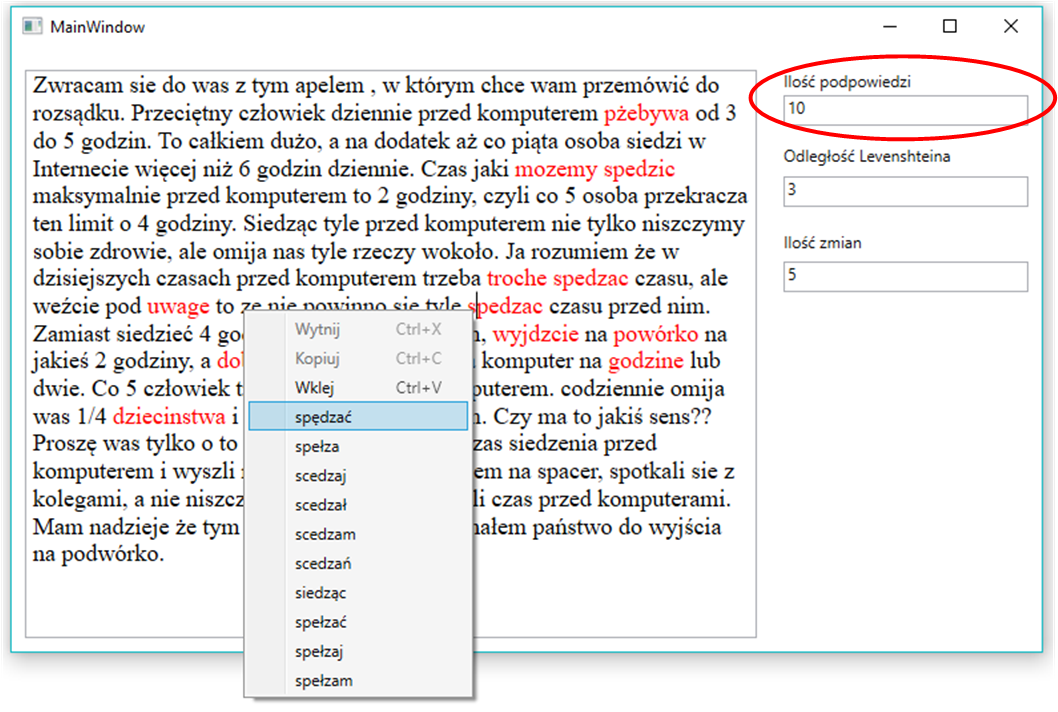
\includegraphics[width=1\linewidth]{rozdzial03/screen3_1.png}
	\caption{Zwiększenie ilości wyświetlanych sugestii}
	\label{fig:interfejs2}
\end{figure}

\begin{figure} [H]
	\centering
	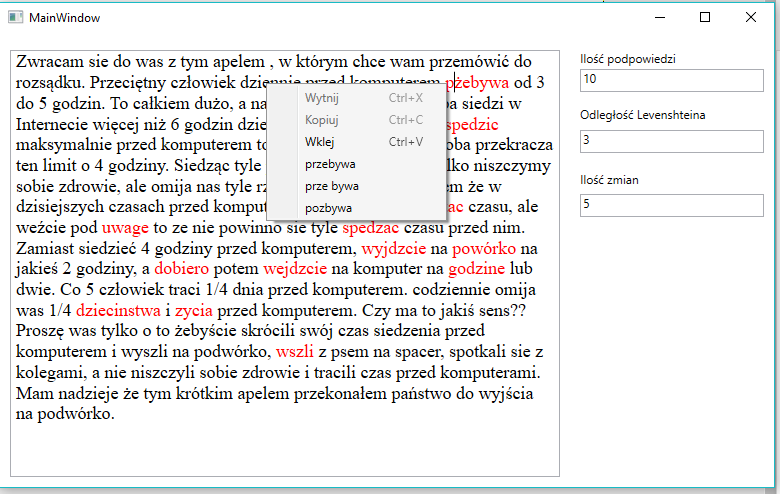
\includegraphics[width=1\linewidth]{rozdzial03/screen4.png}
	\caption{Przykładowy wynik wyszukiwania sugestii dla małej ilości podpowiedzi}
	\label{fig:interfejs3}
\end{figure}

\begin{figure} [H]
	\centering
	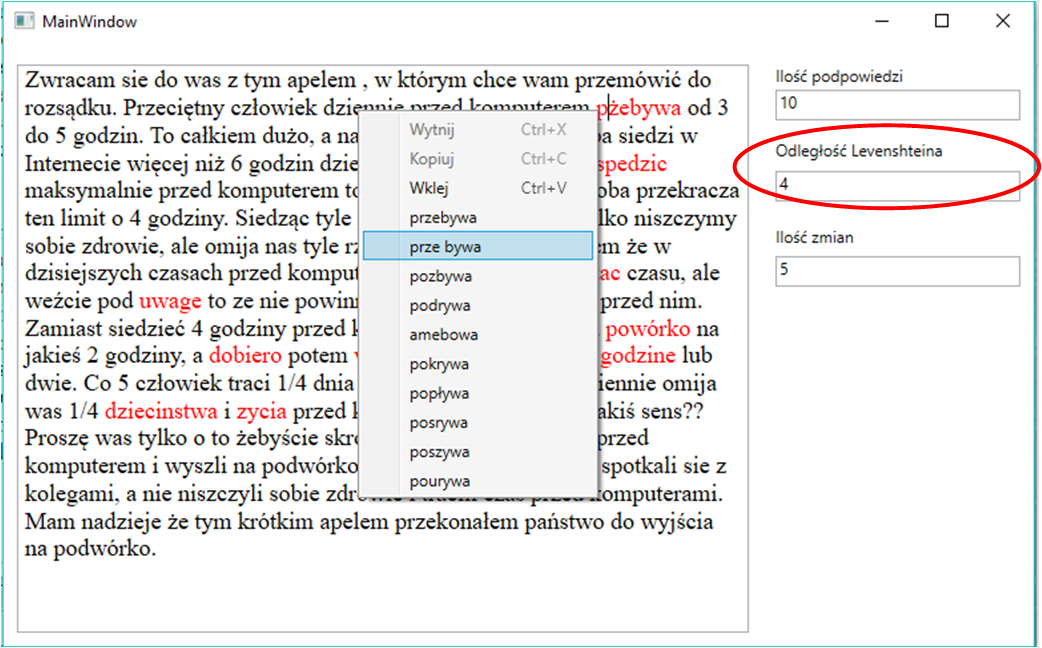
\includegraphics[width=1\linewidth]{rozdzial03/screen5_1.png}
	\caption{Zwiększenie odległości Levenhstaina}
	\label{fig:interfejs4}
\end{figure}

\begin{figure} [H]
	\centering
	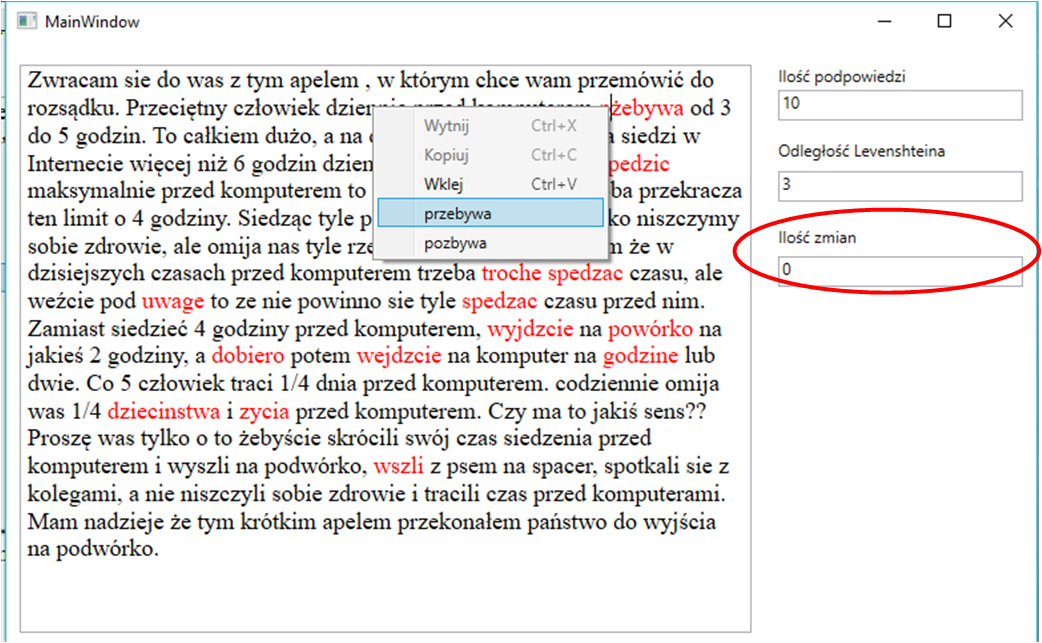
\includegraphics[width=1\linewidth]{rozdzial03/screen6_1.png}
	\caption{Zwiększenie ilości zmian}
	\label{fig:interfejs5}
\end{figure}

Odpowiednio zmieniając parametry znajdujące się w prawej części okna aplikacji można dostosować wyszukiwanie do potrzeb użytkownika. Rysunek \ref{fig:interfejs1} przedstawia przykładowe wyniki wyszukiwania podpowiedzi. Jeśli ilość wyświetlanych wyników nie jest odpowiednia można zmienić ich ilość tak aby uzyskać satysfakcjonujący wynik. Rysunek \ref{fig:interfejs2} przedstawia wpływ zwiększenia ilości wyświetlanych podpowiedzi. Jednocześnie ilość podpowiedzi nie ma wpływu na szybkość działania aplikacji. 

Pozostałe parametry wpływają na podobieństwo sugestii do wprowadzonego błędnie słowa. Na rysunku \ref{fig:interfejs3} został przedstawiony przykładowy wynik wyszukiwania który przy danych parametrach nie wypełnia całej listy podpowiedzi. Na rysunku \ref{fig:interfejs4} zwiększono odległość Levenshteina tak aby uzyskać więcej sugestii. Natomiast na rysunku \ref{fig:interfejs5} całkowicie zminimalizowano wpływ algorytmu podmieniającego znaki tak aby pozbyć się niechcianych podpowiedzi zawierających spacje.
 
\section{Realizacja wybranych funkcjonalności}

\begin{figure} [H]
	\centering
	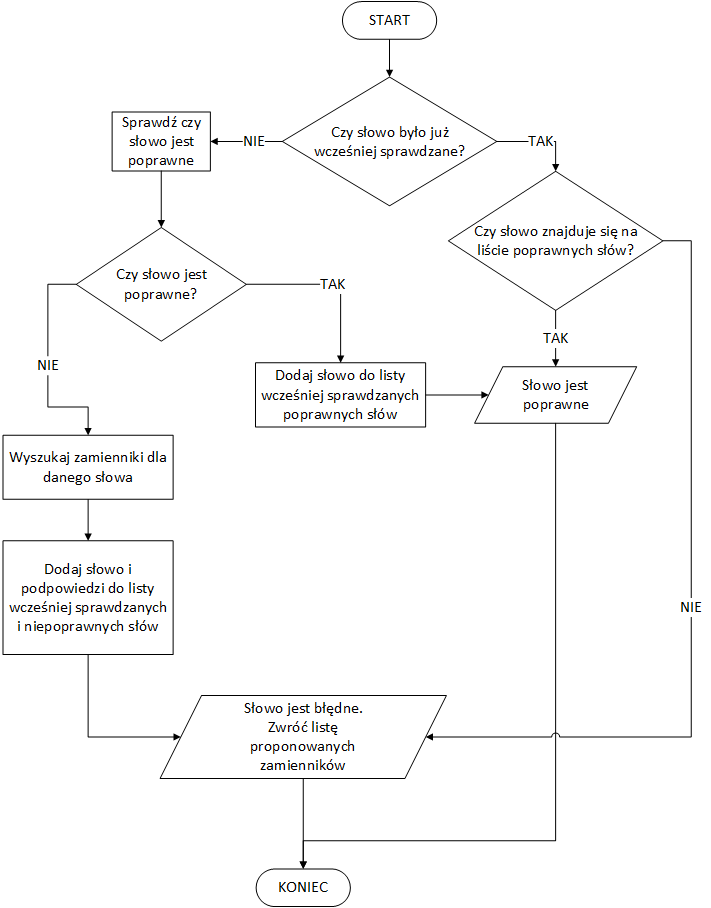
\includegraphics[width=1\linewidth]{rozdzial03/CorectorManager.png}
	\caption{Schemat korekcji tekstu z poziomu interfejsu}
	\label{fig:CorectorManager}
\end{figure}

\newpage

Główną funkcjonalnością aplikacji jest wyszukiwanie a następnie korekcja błędów. Rysunek~\ref{fig:CorectorManager} przedstawia schemat działania algorytmu odpowiedzialnego za powyższe zadanie. 

Początkowo algorytm sprawdza czy dane słowo było już wcześniej wyszukiwane. Jeśli tak to sprawdza czy jest ono na liście poprawnych słów. Jeśli tak to słowo jest poprawne i algorytm kończy pracę. Jeśli nie to sprawdza on listę błędnie wprowadzonych słów i zwraca on podpowiedzi. Jeśli podpowiedzi zostały już raz wyszukane dla danego słowa to zostają one zapisane. Ma to na celu przyspieszenie działania algorytmu ponieważ najwięcej czasu pochłania wyszukiwanie sugestii. 

Jeśli słowo jest wyszukiwane po raz pierwszy następuje sprawdzenie jego poprawności porównując je ze słowami znajdującymi się w słowniku. Jeśli jest poprawne to zostaje ono dodane do listy poprawnych sprawdzanych wcześniej słów i algorytm kończy pracę. Natomiast jeśli słowo jest błędne następuje wyszukiwanie sugestii. Po ich wyszukaniu zostają on zapisane wraz z niepoprawnym wyrazem na liście błędnych słów. Algorytm zwraca listę sugestii i kończy pracę.

Algorytm ten działa dla każdego słowa w osobnym wątku. Ma to za zadnie przyspieszenie działania aplikacji.  

\section{Optymalizacja}
\label{chap:optym}
Słownik użyty w projekcie składa się z blisko trzech milionów haseł. Podczas działania programu słownik ten musi być wielokrotnie przeglądany, zarówno poprzez sprawdzanie każdego wyrazu wpisanego przez użytkownika, jak i badaniu każdej powstałej kombinacji z algorytmu zamiany znaków jak i podziału na wyrazy oraz przy badaniu odległości Levenshteina w najprostszej wersji, każdy badany wyraz powinien mieć mierzoną odległość z każdym wyrazem znajdującym się w słowniku. Przy zwykłym użytkowaniu programu sprowadzałoby się to do wielu milionów operacji, a w związku z faktem iż założono w projekcie, że program ma działać możliwie w czasie rzeczywistym, podjęto próbę rozwiązania problemu z tak dużą liczbą operacji przeglądania całego słownika oraz z ograniczeniem ilości wykonywania obliczania odległości Levenshteina. W poniższych podrozdziałach opisane zostały podjęte w tym zakresie czynności.

\subsection{Serializacja}
Serializacja jest mechanizmem zamiany obiektu zapisywania obiektów, który pozwala na binarny zapis całego drzewa obiektów. Tak zapisany obiekt można w później uruchomić w dowolnym momencie pomijając cały etap tworzenia obiektów, a zastępując go procesem deserializacji, który z reguły powinien trwać szybciej niż proces tworzenia nowych obiektów. \\

W projekcie serializacja użyta została do zapisania klasy odpowiedzialnej za przechowywanie słownika. Przy pierwszym uruchomieniu programu słownik jest wczytywany z pliku tekstowego, a jego hasła są w odpowiedni sposób organizowane (więcej o tym w kolejnym podrozdziale). Dlatego uruchamianie programu i organizowanie słownika za każdym razem od nowa byłoby dość mało optymalne. Klasa z wczytanym słownikiem została zserializowana i zapisana do pliku. Od tego momentu przy każdym ponownym uruchomieniu programu, sprawdzane jest czy ten plik istnieje we wskazanym miejscu i o ile nikt go nie usunął to zostaje wczytany. Operacja trwa o wiele krócej, niż odczyt pliku i organizacja słownika na nowo. \\

Przy wyborze metody serializacji posłużono się artykułem ze strony [\ref{bib:serializ}], z którego to wynika, że jedną z najszybszych metod serializacji i deserializacji odbywa się z wykorzystaniem biblioteki \textit{ProtoBuf}, stworzonej przez firmę \textit{Google}. Metoda ta opera się o zapisywanie stanu klasy do pliku o strukturze XML, a każde pole i właściwość klasy musi zostać wyposażone w specjalny atrybut \textit{[ProtoMember(1)]} , przy czym cyfra podana w nawiasie musi być dla każdego pola unikalna ([\ref{bib:protbuf}]).

\subsection{Organizacja słownika}

Jak już zostało wspomniane w poprzednim podrozdziale, przy pierwszym uruchomieniu słownik jest wczytywany z pliku tekstowego i tworzona jest z niego klasa, która przechowuje słownik ten w odpowiednio zorganizowany sposób, który ułatwia jego przeszukiwanie. 

Hasła są w pamięci przechowywane w dwojaki sposób:
\begin{itemize}
	\item Jako zbiór list, z których każda przechowuje wyrazy o różnej długości oraz są posortowane w sposób alfabetyczny;
	\item Jako zbiór obiektów, z których każdy przechowuje wyrazy o różnej długości oraz rozpoczynające się na różną literę;
\end{itemize}

Pierwszy sposób przechowywania haseł został przystosowany specjalnie dla przeszukiwania słownika, poprzez przeglądanie haseł o wskazanej długości. Jest to szczególnie przydatne dla algorytmu wykorzystującego odległość Levenshteina. Badane słowo ma określoną długość, a zatem prawdopodobnie użytkownikowi również chodziło o słowo podobnej długości. Tak więc nie jest przeszukiwany cały słownik, a jedynie hasła o podobnej długości. W projekcie przyjęto że mogą to być hasła o długości z przedziału od -1 do +1 długości słowa badanego.

Drugi sposób przechowywania haseł został wykorzystany dla pozostałych dwóch algorytmów oraz dla sprawdzania czy dany wyraz znajduje się w słowniku. Przeszukiwanie słownika odbywa się w sposób dużo szybszy, gdyż znana jest długość słowa badanego oraz jego pierwsza litera, a oba te parametry odpowiadają indeksom dwuwymiarowego zbioru w którym przechowywane są hasła.

\subsection{Praca na wielu wątkach}

Jedną z kluczowych funkcjonalności aplikacji jest możliwość pracy równolegle na wielu wątkach jednocześnie. Zostało to zaimplementowane w calu przyspieszenia działania programu. Najbardziej czasochłonną metodą w aplikacji jest wyszukiwanie słów podobnych aby wyświetlić je jako zamienniki błędnych wyrazów. Metoda ta sprawdza każde słowo w słowniku korzystając z jednego z trzech wcześniej opisanych algorytmów. Ponieważ ogranicza się ona do jednego słowa możliwe było zrównoleglenie tego procesu tak aby sprawdzać wiele słów jednocześnie. Dzięki zastosowaniu takiego rozwiązania szybkość działania aplikacji została znacząco zwiększona.


	\chapter{Podsumowanie}

Aplikacja stworzona na potrzeby projektu spełnia wszystkie cele oraz założenia projektowe. Pozwala ona na sprawdzenie dowolnego tekstu w języku polskim wpisanego przez użytkownika. Użytkownik ma możliwość wstawienia w każde z błędnych słów innego zasugerowanego przez system. Dzięki zoptymalizowaniu algorytmów wyszukiwania jak i interfejsu użytkownika wyszukiwanie sugestii odbywa się w czasie rzeczywistym. Dzięki zastosowaniu słownika w postaci pliku tekstowego jego modyfikacja w formie dodawania kolejnych wyrazów jest bardzo prosta. \\ 

W celu wyszukiwania jak najtrafniejszych zamienników dla błędnie napisanych słów zaimplementowano trzy algorytmy:
\begin{itemize}
	\item Odległość Levenshteina - oblicza on odległość edycyjną dwóch porównywanych napisów, odległość ta wyrażana jest przez liczbę operacji podstawowych. Jednak konieczność przeglądania całego słownika, w dość znacznym stopniu obciąża procesor, dlatego też w projekcie zastosowano wyłącznie porównywanie słów o podobnej długości (plus minus jeden znak).
	\item Zamiana znaków - algorytm ten zamienia ciągi znakowe odpowiadające częstym błędom ortograficznym w języku polskim i na tej podstawie utworzyć może wiele kombinacji i w pewnym stopniu uzupełnia uproszczenie zastosowane w przypadku użycia odległości Levenstheina, dla wybranych fragmentów słownika.
	\item Podział na wyrazy - algorytm ten przeciwdziała częstym błędom w piśmie komputerowym, wynikającym z braku wciśnięcia spacji. 
\end{itemize}

Dzięki takiemu rozwiązaniu program dobrze radzi sobie niezależnie od rodzaju błędu jaki popełnił użytkownik.

Aplikacja została napisana w języku C\# dlatego jest przeznaczona na komputery z systemem Windows. Korzystanie z niej nie wymaga instalacji. Dodatkowo jest to niezależna aplikacja, która do działania nie wymaga dodatkowych bibliotek.
	\addcontentsline{toc}{chapter}{Literatura} %utworzenie w spisie treści pozycji Bibliografia
	\pagestyle {empty}

\vspace*{1.3cm}

{\Huge\textbf{Literatura}}

\vspace*{1cm}

\begin{enumerate}[\lbrack 1\rbrack]
	\item Anonim G. i in., \textit{Kronika polska}, T.1: \textit{Kronika i czyny książąt czyli władców polskich}, Gniezno 1115
\end{enumerate}


	
	%\pagestyle {empty}

\vspace*{1.3cm}

{\Huge\textbf{Literatura}}

\vspace*{1cm}

\begin{enumerate}[\lbrack 1\rbrack]
	\item Anonim G. i in., \textit{Kronika polska}, T.1: \textit{Kronika i czyny książąt czyli władców polskich}, Gniezno 1115
\end{enumerate}


	%\bibliography{bibliografia} % wstawia bibliografię korzystając z pliku bibliografia.bib - dotyczy BibTeXa, jeżeli nie korzystamy z BibTeXa należy użyć otoczenia thebibliography
	
\end{document}